% Figure 4.8  (label fig:cfghub_sys)
% Caption: System-Level Integration of the Function Switch Controller.
% Extracted standalone source of the TikZ figure embedded in MARS_碩士論文.tex
% Compile: pdflatex fig4.8_cfghub_sys.tex
\documentclass[border=6pt]{standalone}
\usepackage{tikz}
\usetikzlibrary{shapes.geometric, arrows.meta, positioning, fit, backgrounds, calc, decorations.pathreplacing}
\begin{document}
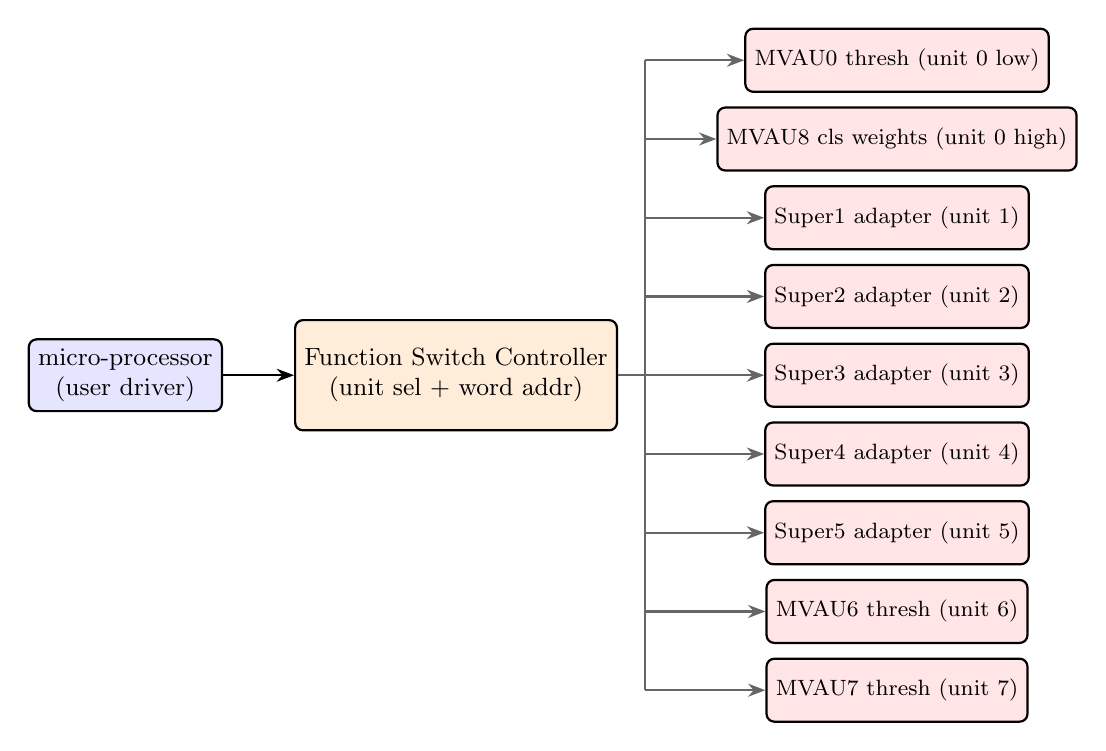
\begin{tikzpicture}[
    font=\small,
    ps/.style={rectangle, draw, thick, rounded corners=1mm, fill=blue!10, minimum width=2.2cm, minimum height=0.9cm, align=center},
    hub/.style={rectangle, draw, thick, rounded corners=1mm, fill=orange!15, minimum width=3.4cm, minimum height=1.4cm, align=center},
    mod/.style={rectangle, draw, thick, rounded corners=1mm, fill=red!10, minimum width=2.0cm, minimum height=0.8cm, align=center, font=\footnotesize},
    arr/.style={-{Stealth[length=2.2mm]}, thick}
]
\node[ps] (ps) at (0,0) {micro-processor\\(user driver)};
\node[hub] (hub) at (4.2,0) {Function Switch Controller\\(unit sel + word addr)};
\draw[arr] (ps.east) -- (hub.west);

\node[mod] (u0l) at (9.8, 4.0) {MVAU0 thresh (unit 0 low)};
\node[mod] (u0h) at (9.8, 3.0) {MVAU8 cls weights (unit 0 high)};
\node[mod] (s1)  at (9.8, 2.0) {Super1 adapter (unit 1)};
\node[mod] (s2)  at (9.8, 1.0) {Super2 adapter (unit 2)};
\node[mod] (s3)  at (9.8, 0)   {Super3 adapter (unit 3)};
\node[mod] (s4)  at (9.8,-1.0) {Super4 adapter (unit 4)};
\node[mod] (s5)  at (9.8,-2.0) {Super5 adapter (unit 5)};
\node[mod] (u6)  at (9.8,-3.0) {MVAU6 thresh (unit 6)};
\node[mod] (u7)  at (9.8,-4.0) {MVAU7 thresh (unit 7)};

\draw[black!60, thick] (hub.east) -- (6.6,0);
\draw[black!60, thick] (6.6,4.0) -- (6.6,-4.0);
\foreach \t in {u0l, u0h, s1, s2, s3, s4, s5, u6, u7} {
    \draw[arr, black!60] (6.6,0 |- \t.west) -- (\t.west);
}
\end{tikzpicture}
\end{document}
